\documentclass[11pt]{article}
\usepackage{graphicx}
\usepackage{amssymb}
\usepackage{bm}
\usepackage{mathtools}
\usepackage{amsmath}
\usepackage{commath}
\usepackage{amsthm}
\usepackage{enumitem}
\usepackage{float} 
\usepackage{array}
\usepackage{outlines}
\usepackage{setspace}
\usepackage[colorinlistoftodos]{todonotes}
\definecolor{green}{rgb}{0.4, 0.69, 0.2}
\definecolor{asparagus}{rgb}{0.53, 0.66, 0.42}
\definecolor{blue}{rgb}{0.0, 0.53, 0.74}
\definecolor{terracotta}{HTML}{e2725b}
\definecolor{mocassin}{HTML}{FFE4B5}
\definecolor{coral}{HTML}{FFAA80}
\setlist[enumerate,1]{label=\roman*)}
\setlist[enumerate,2]{label=\alph*)}
\newtheorem{theorem}{Theorem}
\newtheorem{corollary}{Corollary}
\newtheorem{lemma}{Lemma}
\newtheorem{remark}{Remark}
\newtheorem{definition}{Definition}
\newtheorem{prop}{Proposition}
\newcommand*\diff{\mathop{}\!\mathrm{d}}
\usepackage{tikz}
\usetikzlibrary{arrows,shapes,trees, calc}
\usepackage{graphicx}
\usepackage{subfig}

\usepackage{xcolor}
\definecolor{grey}{rgb}{0.9,0.9,0.9}

\begin{document}

\begin{titlepage}
	\colorbox{grey}{
		\parbox[t]{0.93\textwidth}{
			\parbox[t]{0.91\textwidth}{
				\raggedleft
				\fontsize{50pt}{80pt}\selectfont
				\vspace{0.7cm}
				{\fontfamily{qhv}\selectfont PhD final report} \\
				\vspace{0.7cm}
			}
		}
	}
	\vfill
	\parbox[t]{0.93\textwidth}{
		\raggedleft
		\large
		{\Large N\'{o}ra Juh\'{a}sz}\\[4pt]
		DISIM\\
		University of L'Aquila\\[4pt]
		\texttt{\Large Supervisor: Prof. D. Donatelli}\\
		
		\hfill\rule{0.2\linewidth}{1pt}
	}
\end{titlepage}

\newpage
\tableofcontents

\newpage

\section{Research activity: Mathematical modelling of the polluted atmosphere}

\subsection{The scope of this project in a nutshell}

The key aspects of capturing the dynamics of either water flow in oceanography or atmospheric changes in meteorology are the following two fundamental concepts that underlie many modern asymptotic models aiming to describe them. The first one is that both above mentioned phenomena can be viewed as a fluid dynamics process, and as such, they are best described by the Navier-Stokes equations. The second is the notion of the so-called shallow domains. This latter is a widely used concept in the field of large-scale geophysical fluids and its main idea is to take advantage of their approximately flat structure when modelling them with the Navier-Stokes equations, leading to the classic hydrostatic approximation of the Navier-Stokes equations. We use the

\[ \epsilon = \frac{\text{characteristic depth}}{\text{characteristic width}} \]

aspect ratio and the fact that, as the above described general ideas suggest, it is natural to consider asymptotic models and to take the limit model as $\epsilon$ goes to zero.

In this work we couple the Navier-Stokes equations representing fluid velocity with a convection-diffusion equation describing air pollutant concentration, and show that the solutions of the complete coupled system (anisotropic equations) on a shallow domain are in fact "close" to the solutions of the hydrostatic model. In more detail, we verify a rigorous connection between two fundamental models, namely the anisotropic and hydrostatic models, and show that they are interwoven on the level of both weak and strong solutions --- providing with this a generalised verification of meteorological models based on the hydrostatic approximation. The main novelty of this work is the elaboration of the convergence results in two different coordinate systems, in particular in the mathematically more challenging, so-called downwind-matching coordinate system, and the addition of the concentration function to the model --- important convergence results for the velocity functions in geophysical coordinates had been available previously, see \cite{azerad2001mathematical} and \cite{li2019primitive}. We also perform numerical simulations in order to have a visual affirmation of the fact of the convergence.

\subsection{Weak convergence in geophysical coordinates}

Firstly, we describe a self-contained model representing the atmospheric flow combined with the pollution effects and we investigate the asymptotic behaviour of the weak solutions of this model. The model utilises classical concepts as its foundation and it merges them with relatively new or more specific ideas. On the one hand, we use general and well-known approaches such as the wind flow being modelled by the incompressible anisotropic Navier-Stokes equations, and using a convection-diffusion equation to describe the pollution effect. On the other hand, the model also incorporates notions like using a Gaussian pulse as a source term (\cite{zhuk2016source}) for the case of weak solutions, and rescaling the diffusivity parameters according to the largely different horizontal and vertical scales (similarly to the way the viscosity terms are scaled in \cite{azerad2001mathematical}).

We begin by choosing a coordinate system, set the domain and an appropriate set of equations describing both atmosphere motions and the effect of pollution. We ignore large scale effects such as the curvature of the Earth. For describing the effect of pollution we use a continuity equation written in Cartesian coordinates for the concentration: we fix a local Cartesian coordinate system where the axes are independent from the wind ($x, y$ and $z$ are oriented towards east, north, and upwards, respectively). A different choice of coordinates is described in detail later.

The domain we consider is a local slice of the atmosphere filled with homogeneous incompressible air and a pollutant, and it is defined by the set

\begin{equation}
  \Omega_{\epsilon} = \{(x,y,z) \in \mathbb{R}^3 ; (x,y) \in \omega, 0 < z < \epsilon h(x,y) \},
\end{equation}

where $\epsilon$ incorporates the shallowness of the domain.

The equations governing the air velocity $\mathbf{v}, $ the pressure $q$ and the pollution concentration $P$ in the atmosphere are the incompressible Navier-Stokes equations combined with an advection-diffusion equation. We use different viscosities according to vertical or horizontal directions, and the density is taken to be identically equal to one:

\begin{equation} \label{originalEQ-V}
  \partial_t \mathbf{v} + (\mathbf{v} \cdot \nabla)\mathbf{v} -\Delta_{\nu} \mathbf{v} + \nabla q + 2 \mathbf{w} \times \mathbf{v}= \mathbf{g} \text{ in } \Omega_{\epsilon} \times (0,T)
\end{equation}
    
\begin{equation} \label{originalEQ-I}
  \nabla \cdot \mathbf{v} = 0 \text{ in } \Omega_{\epsilon} \times (0,T)
\end{equation}
    
\begin{equation} \label{diffusive}
  \partial_t P + \mathbf{v} \cdot \nabla P = \nabla \cdot (\mathbf{K} \nabla P) + Q,
\end{equation}

where $P$ is the pollution concentration and $\mathbf{K}$ is the $3 \times 3$ diffusion matrix.

Now, we perform a vertical scaling to make the domain independent of $\epsilon.$

    \[x=x_1, \quad y=x_2, \quad z=\epsilon x_3. \]
    
We have the following new, $\epsilon$ - independent domain
    
    \[ \Omega =  \{(x_1,x_2,x_3) \in \mathbb{R}^3 ; (x_1,x_2) \in \omega, 0 < x_3 < h (x_1 , x_2) \}.\]
    
The corresponding scaling regarding the kinematic, pressure and viscosity terms are
     
    \[v_1 = u_1^{\epsilon}, \quad v_2 = u_2^{\epsilon}, \quad v_3 = \epsilon u_3^{\epsilon}, \quad p = p^{\epsilon}, \]
    \[\nu_x = \nu_1, \quad \nu_y = \nu_2 , \quad \nu_z = \epsilon ^ 2\nu_3. \]
    
Note that from this point we have $\nabla = (\partial_1, \partial_2, \partial_3) $ and $ \Delta_\nu = \nu_1 \partial^2_{11} + \nu_2 \partial^2_{22}  + \nu_3 \partial^2_{33} $. 
    
We use an analogous rescaling methodology for the diffusivity constants in (\ref{diffusive}),
    
\begin{gather}
 \begin{bmatrix} K_{xx} & K_{xy} & K_{xz} \\ K_{yx} & K_{yy} & K_{yz} \\ K_{zx} & K_{zy} & K_{zz} \end{bmatrix}
 =
  \begin{bmatrix}
    M_{11} & M_{12} & \epsilon M_{13} \\ M_{21} & M_{22} & \epsilon M_{23} \\ \epsilon M_{31} & \epsilon M_{32} & \epsilon^2 M_{33}
  \end{bmatrix}
\end{gather}

Here we emphasise that the diffusivity matrix $\mathbf{M}$ is assumed to have the coercivity property.

Finally we obtain the rescaling equations for the pollution concentration and the source term:

    \[ P = \frac{1}{\epsilon} C^\epsilon, \quad Q = \frac{1}{\epsilon} S^\epsilon. \]
    
As for the source term, we enable requirements of different strength depending on whether we consider the case of weak or strong solutions.

In this case, investigating weak convergence, we will use localised point sources as suggested in \cite{zhuk2016source} and we use what is called a parametrised nascent delta function (a Gaussian impulse, specifically) to describe the source term $S^\epsilon$:

\begin{equation} \label{sourcedefinition}
  S^\epsilon = I H(t-t_s) \gamma \epsilon^{-3} e ^ {\frac{-(\mathbf{x}-\mathbf{x_s})^2}{\epsilon^2}},
\end{equation}

while in the limit model the source term $S$ naturally stands for the $\delta$ distribution.
    
Putting the previously described rescaling terms together to the original equations (\ref{originalEQ-V})-(\ref{diffusive}), we arrive to the merged anisotropic equations of the polluted atmosphere above inland surface:
  
    \begin{equation} \label{ANSC1}
    \partial_t u^\epsilon _1 + \mathbf{u}^\epsilon \cdot \nabla u^\epsilon _1 -\Delta_\nu u^\epsilon _1 -\alpha u_2^\epsilon + \epsilon \beta u_3^\epsilon + \partial_1 p^\epsilon = 0 \text{ in } \Omega \times (0,T)
    \end{equation}
    
    \begin{equation} \label{ANSC2}
    \partial_t u_2^\epsilon + \mathbf{u}^\epsilon \cdot \nabla u_2^\epsilon -\Delta_\nu u_2^\epsilon + \alpha u_1^\epsilon + \partial_2 p^\epsilon = 0 \text{ in } \Omega \times (0,T)
    \end{equation}
    
    \begin{equation} \label{ANSC3}
    \epsilon^2 \{  \partial_t u_3^\epsilon + \mathbf{u}^\epsilon \cdot \nabla u_3^\epsilon -\Delta_\nu u_3^{\epsilon} \} - \epsilon \beta u_1^\epsilon + \partial_3 p^\epsilon = 0 \text{ in } \Omega \times (0,T)
    \end{equation}
    
    \begin{equation} \label{ANSC4}
    \nabla \cdot \mathbf{u}^\epsilon= 0 \text{ in } \Omega \times (0,T)
    \end{equation}
    
    \begin{equation} \label{ANSC5}
    \partial_t C^\epsilon + \mathbf{u^\epsilon} \cdot \nabla C^\epsilon = \nabla \cdot (\mathbf{M} \nabla C^\epsilon) + S^\epsilon \text{ in } \Omega \times (0,T)
    \end{equation}

The initial condition for the velocity and the pollution concentration are
    
    \begin{equation} \label{ANSC7}
    \mathbf{u}^\epsilon (\cdot, t = 0) = \mathbf{u}_0, \quad C^\epsilon (\cdot, t=0) = C_0  \quad \text{ in } \Omega.
    \end{equation}
    
To make the above set of equations complete, we need to assign the boundary conditions, which we set as shown by the graph below.

\begin{figure}[!h]
  \centering
  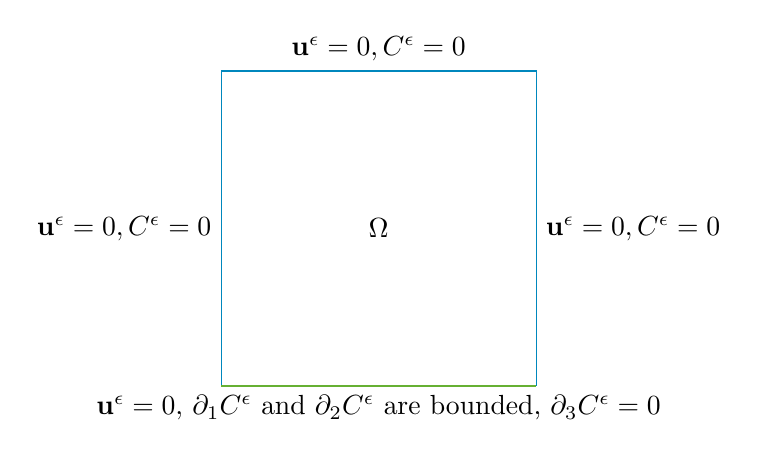
\begin{tikzpicture}
  
    \draw[blue] (0,0) -- (2,0) -- (4,0) -- (4,2) -- (4,4) -- (2,4) -- (0,4) -- (0,2) -- (0,0);
    \draw[green, thick] (0,0) -- (4,0);
    
    \draw (2,2)node{$\Omega$};
    \draw (2,0)node[below] {$\mathbf{u^\epsilon} = 0,$ $ \partial_1 C^\epsilon$ and $ \partial_2 C^\epsilon$ are bounded, $\partial_3 C^\epsilon = 0$};
    \draw (4,2)node[right] {$\mathbf{u^\epsilon} = 0, C^\epsilon=0 $};
    \draw (2,4)node[above] {$\mathbf{u^\epsilon} = 0, C^\epsilon=0 $};
    \draw (0,2)node[left] {$\mathbf{u^\epsilon} = 0, C^\epsilon=0 $};
    
  \end{tikzpicture}
\end{figure}
  
    \begin{equation} \label{ANSC8}
      \begin{split}
        & \mathbf{u}^\epsilon = 0 \text{ on } \Gamma \times (0,T), \\
        &C^\epsilon = 0 \text{ on } ( \Gamma_U \cup \Gamma_L) \times (0,T), \\
        & \partial_1 C^\epsilon = \sigma_1, \partial_2 C^\epsilon = \sigma_2,\ \partial_3 C^\epsilon= 0 \text{ on } \Gamma_G \times (0,T), \\
        & \boldsymbol{\sigma} = (\sigma_1, \sigma_2, 0) \in L^2(0,T; \Gamma_G)\\
      \end{split} \raisetag{40pt}
    \end{equation}

If we assume $\mathbf{u}^\epsilon = O(1)$, then neglecting the $\epsilon^2$ and $\epsilon$ in the anisotropic equations, we formally arrive to the hydrostatic Navier-Stokes equations (i.e., primitive equations) combined with pollution.

    \begin{equation} \label{HNSC1}    
    \partial_t u_1 + \mathbf{u} \cdot \nabla u_1 - \Delta_\nu u_1 -\alpha u_2 + \partial_1 p = 0 \text{ in } \Omega \times (0,T)
    \end{equation}
    
    \begin{equation} \label{HNSC2}   
    \partial_t u_2 + \mathbf{u} \cdot \nabla u_2 - \Delta_\nu u_2 -\alpha u_1 + \partial_2 p = 0 \text{ in } \Omega \times (0,T)
    \end{equation}
    
    \begin{equation} \label{HNSC3}   
    \partial_3 p = 0 \text{ in } \Omega \times (0,T)
    \end{equation}
    
    \begin{equation} \label{HNSC4}   
    \nabla \cdot \mathbf{u} = 0 \text{ in } \Omega \times (0,T)
    \end{equation}
    
    \begin{equation} \label{HNSC5}   
    \partial_t C + \mathbf{u} \cdot \nabla C = \nabla \cdot (\mathbf{M} \nabla C) + S \text{ in } \Omega \times (0,T)
    \end{equation}
    
    \begin{equation} \label{HNSC6}   
    u_1 = u_2 = u_3 n_3 = 0 \text{ on } \Gamma \times (0,T)
    \end{equation}
    
    \begin{equation} \label{HNSC7}   
    u_i (\cdot, t=0) = u_{0 i}, C (\cdot, t=0) = C_0 \text{ in } \Omega, \text{$i$ = 1,2}
    \end{equation}
    
    \begin{equation} \label{HNSC8}
      \begin{split}
        &C = 0 \text{ on } ( \Gamma_U \cup \Gamma_L) \times (0,T), \\
        & \partial_1 C = \sigma_1, \partial_2 C = \sigma_2, \partial_3  C = 0, \boldsymbol{\sigma} = (\sigma_1, \sigma_2, 0) \in L^2(0,T; \Gamma_G)\\
      \end{split}
    \end{equation}

\subsubsection{Theoretical justification of the hydrostatic model on the level of weak solutions}

In this subsection we write down the weak formulations of the two different systems in geophysical coordinates, and provide the main steps of the proof that shows that any weak solution of the anisotropic system converges to a weak solution of the hydrostatic system as $\epsilon$ goes to zero.

\subsubsection{Visualisation of the weak convergence result using \textbf{FEniCS}}

We visualise the weak convergence result with \textbf{FEniCS} --- a software with the finite element method at its core.

The major challenge in numerically approaching the tendency of the solutions as $\epsilon$ goes to zero is the disappearing dependence of the scheme on certain terms. Picard iterations and the Chorin method for example are widely used methods in the field of the (complete) Navier-Stokes equations, but once we introduce an $\epsilon$ into the equations, these schemes "collapse" rather quickly as this parameter becomes zero.

In the \textbf{Chorin method} the $u \nabla u_1 v_1$ nonlinear term is replaced by

\texttt{inner(u\_prev, grad(u\_prev1)) * v1 * dx},

where essentially we don't have any unknowns at all anymore. The first step of the Chorin method calculates a tentative velocity. The \texttt{u1, u2, u3} functions are the unknowns, while \texttt{u\_prev} is calculated from the previous time step. It is easy to see in the following pseudo code that the scheme depends on \texttt{\textcolor{terracotta}{u3}} only through $\epsilon^2.$

\texttt{
\\
F = (1/dt)((u\_H - u\_prev\_H)*v\_H + eps*eps*(\textcolor{terracotta}{u3} - u\_prev3)*v3 ) + \\
inner(u\_prev, grad(u\_prev\_H)) * v\_H\\
 + eps*eps*inner(u\_prev, grad(u\_prev3)) * v3 + \\
 inner(grad(u\_H),grad(v\_H)) + eps*eps*inner(grad(\textcolor{terracotta}{u3}),grad(v3)) \\
}

Similarly, the linearisation technique of \textbf{Picard iterations} also lead to a problematic scheme:

\texttt{
\\
a = inner(\textcolor{blue}{u}, grad(u\_k\_H)) * v\_H + eps*eps*inner(u, grad(\textcolor{green}{u\_k3})) * v3 + \\
inner(grad(u\_H),grad(v\_H)) + eps*eps*inner(grad(u3),grad(v3)),\\
}

where the dependence on \texttt{u\_k3} decreases with $\epsilon^2.$ This suggests in our case to avoid linearisation techniques and conserve the nonlinear nature of the problem, which can improve the dependence of the scheme on its variables.

We consider a simplified model that still contains this fundamental phenomena (the decreasing dependence as $\epsilon \to 0$) in space. Thus, we consider

\begin{enumerate}
  \item a stationary case,
  \item without the Coriolis term,
  \item we make the two horizontal dimensions fall into one. It is easy to see that in a theoretical point of view, and also in terms of proving regularities, the two horizontal dimensions are not different. The problem consists of having $n-1$ dimensions with $\mathcal{O}(1)$ scale, and $1$ dimension with $\mathcal{O}(\epsilon)$ scale. Instead of the $n-1$ dimensions we can use 1 for quicker computations and easier visualisation, and
  \item in order to obtain better results, we take the same equations, but we use them as equations describing water flow. The convergence result is the same, the boundary conditions are slightly different, and using wind traction over the water surface helps to highlight the point of our result.
\end{enumerate}

Taking these ideas into account, we will use the Newton solver in the following way:

\texttt{
\\
F = inner(u, grad(u1)) * v1 * dx + inner(grad(u1),grad(v1)) * dx + eps*eps*inner(u, grad(u3)) * v3 * dx\\
+ eps*eps*inner(grad(u3),grad(v3)) * dx - p * div(v) * dx + q * div(u) * dx - inner(theta, v) * ds(1),\\
}

and we apply

\texttt{
\\
problem = NonlinearVariationalProblem(F, up\_, bcu, J)\\
solver  = NonlinearVariationalSolver(problem), \\
}

to the \texttt{F} scheme. Note that here, instead of $\texttt{u\_H}$ we denote the horizontal velocity by $\texttt{u1}$ to express that we use the dimension reduction idea for the horizontal velocity during the computations.

Similarly, for the hydrostatic model we use an analogous scheme where the $\epsilon$- including terms are missing.

The most important difference is that while for the anisotropic model we use a finite element space of degree $2$ for the vertical velocity, for the case of the hydrostatic scheme we use a degree $1$ space for the same variable. This phenomena is yet to be investigated further, but we have observed that the hydrostatic scheme, which contains significantly less information about the vertical velocity, does not converge for the case of a degree $2$ vertical space (unless the hydrostatic Newton solver is initialised with the anisotropic solution obtained for very small $\epsilon$, with slightly less strict error tolerance values).

To summarise, we have been able to visualise the convergence of the weak solutions for the following cases:

\begin{itemize}
  \item Anisotropic scheme with degree $2$ horizontal velocity space and degree $2$ vertical velocity space: works until $\epsilon = \exp{-7},$ and visibly approaches the solution of the hydrostatic scheme obtained for degree $2$ horizontal space and degree $1$ vertical space.
  \item The hydrostatic scheme with (2,2) space degrees initialised with the anisotropic solution obtained with the $\exp{-7} $ $\epsilon$ value as an initial guess: converges immediately. In this case the Newton solver verifies in a single step that the initial guess, i.e. the solution for the anisotropic model for a very small $\epsilon$ value is in fact a solution for the hydrostatic model.
  \item Remark: The anisotropic scheme with degrees (2,1) is theoretically unadvisable to use as the so called lim-sup stability condition is not satisfied.
\end{itemize}

In the following we include some of the visual results obtained with \textbf{FEniCS}.

\newpage

\subsubsection{The tendency of the pressure solution}

\begin{figure}[H]
\centering
\begin{minipage}{0.5\textwidth}
  \centering
  
\includegraphics[width=0.9\linewidth]{results2D_H_V/images/pressure_anis_1_0000000}
  \captionof{figure}{$\epsilon = 1.0000000.$}
\end{minipage}%
\begin{minipage}{0.5\textwidth}
  \centering
  
\includegraphics[width=0.9\linewidth]{results2D_H_V/images/pressure_anis_0_5000000}
  \captionof{figure}{$\epsilon = 0.5000000.$}
\end{minipage}
\end{figure}

\begin{figure}[H]
\centering
\begin{minipage}{0.5\textwidth}
  \centering
  
\includegraphics[width=0.9\linewidth]{results2D_H_V/images/pressure_anis_0_0625000}
  \captionof{figure}{$\epsilon = 0.0625000.$}
\end{minipage}%
\begin{minipage}{0.5\textwidth}
  \centering
  
\includegraphics[width=0.9\linewidth]{results2D_H_V/images/pressure_anis_0_0312500}
  \captionof{figure}{$\epsilon = 0.0312500.$}
\end{minipage}
\end{figure}

\begin{figure}[H]
\centering
\begin{minipage}{0.5\textwidth}
  \centering
  
\includegraphics[width=0.9\linewidth]{results2D_H_V/images/pressure_anis_0_0156250}
  \captionof{figure}{$\epsilon = 0.0156250.$}
\end{minipage}%
\begin{minipage}{0.5\textwidth}
  \centering
  
\includegraphics[width=0.9\linewidth]{results2D_H_V/images/pressure_hydr}
  \captionof{figure}{Hydrostatic model.}
  \label{fig:test2}
\end{minipage}
\end{figure}

\newpage

\subsubsection{The tendency of the horizontal velocity solution}

\begin{figure}[H]
  \centering
  
\includegraphics[width=3in]{results2D_H_V/images/velocity_h_anis_1_0000000}
  \caption{$\epsilon = 1.0000000.$}
\end{figure}

\begin{figure}[H]
  \centering
  
\includegraphics[width=3in]{results2D_H_V/images/velocity_h_anis_0_0078125}
  \caption{$\epsilon = 0.0078125.$}
\end{figure}

\begin{figure}[H]
  \centering
  
\includegraphics[width=3in]{results2D_H_V/images/velocity_h_hydr}
  \caption{Hydrostatic model.}
\end{figure}

\newpage

\subsubsection{The tendency of the vertical velocity solution}

\begin{figure}[H]
\centering
\begin{minipage}{0.5\textwidth}
  \centering
  
\includegraphics[width=0.9\linewidth]{results2D_H_V/images/velocity_v_anis_1_0000000}
  \captionof{figure}{$\epsilon = 1.0000000.$}
\end{minipage}%
\begin{minipage}{0.5\textwidth}
  \centering
  
\includegraphics[width=0.9\linewidth]{results2D_H_V/images/velocity_v_anis_0_5000000}
  \captionof{figure}{$\epsilon = 0.5000000.$}
\end{minipage}
\end{figure}

\begin{figure}[H]
\centering
\begin{minipage}{0.5\textwidth}
  \centering
  
\includegraphics[width=0.9\linewidth]{results2D_H_V/images/velocity_v_anis_0_2500000}
  \captionof{figure}{$\epsilon = 0.2500000.$}
\end{minipage}%
\begin{minipage}{0.5\textwidth}
  \centering
  
\includegraphics[width=0.9\linewidth]{results2D_H_V/images/velocity_v_anis_0_1250000}
  \captionof{figure}{$\epsilon = 0.1250000.$}
\end{minipage}
\end{figure}

\begin{figure}[H]
\centering
\begin{minipage}{0.5\textwidth}
  \centering
  
\includegraphics[width=0.9\linewidth]{results2D_H_V/images/velocity_v_anis_0_0625000}
  \captionof{figure}{$\epsilon = 0.0625000.$}
\end{minipage}%
\begin{minipage}{0.5\textwidth}
  \centering
  
\includegraphics[width=0.9\linewidth]{results2D_H_V/images/velocity_v_anis_0_0312500}
  \captionof{figure}{$\epsilon = 0.0312500.$}
\end{minipage}
\end{figure}

\begin{figure}[H]
\centering
\begin{minipage}{0.5\textwidth}
  \centering
  
\includegraphics[width=0.9\linewidth]{results2D_H_V/images/velocity_v_anis_0_015625}
  \captionof{figure}{$\epsilon = 0.0156250.$}
\end{minipage}%
\begin{minipage}{0.5\textwidth}
  \centering
  
\includegraphics[width=0.9\linewidth]{results2D_H_V/images/velocity_v_anis_0_0078125}
  \captionof{figure}{$\epsilon = 0.0078125.$}
\end{minipage}
\end{figure}

\begin{figure}[H]
\centering
\begin{minipage}{0.5\textwidth}
  \centering
  
\includegraphics[width=0.9\linewidth]{results2D_H_V/images/velocity_v_anis_1_19e-07}
  \captionof{figure}{$\epsilon = 1.19 \exp{(-7)}.$}
\end{minipage}%
\begin{minipage}{0.5\textwidth}
  \centering
  
\includegraphics[width=0.9\linewidth]{results2D_H_V/images/velocity_v_hydr}
  \captionof{figure}{Hydrostatic model.}
\end{minipage}
\end{figure}

\subsection{Weak convergence in downwind-matching coordinates}

Weak convergence in downwind-matching coordinates

\subsection{Strong convergence in downwind-matching coordinates}

Strong convergence

\newpage

\nocite{*}
\bibliographystyle{abbrv}
\bibliography{bibliography-report}

\newpage

\section{Attended courses}

\subsection{Academic year 2016 / 2017}

\begin{itemize}

  \item Numerical Analysis 2 --- Prof. Guglielmi (University of L'Aquila)
  \item High Performance Parallel Computing --- Prof. Shcherbatyy, Prof. Protasov, Prof. Khapko, Prof. Pera (University of L'Aquila)
  \item Introduction to Finite Elements Method --- Prof. Boffi (GSSI)
  \item Decay property for hyperbolic systems with dissipation --- Prof. Kawashima (GSSI)
  \item Advanced Topics on Numerical Methods --- Prof. Guglielmi (GSSI)
  \item Introduction to the Incompressible Navier-Stokes equation --- Prof. Marcati (GSSI)

\end{itemize}

\subsection{Academic year 2017 / 2018}

\begin{itemize}

  \item Physics of the atmosphere --- Prof. G. Curci, Prof. G. Redaelli (University of L'Aquila)
  \item Numerical methods for hyperbolic problems --- Prof. G. Russo (GSSI)
  
\end{itemize}

\newpage

\section{Conferences and summer schools}

\begin{itemize}
  \item Summer School on Reduced Order Methods in Computational Fluid Dynamics, SISSA, Trieste, July 8 - 12, 2019
  \item The XVIII Italian Meeting on Hyperbolic Equations, University of Palermo, Palermo, May 15 - 17, 2019
  \item The Finite Element Method Using deal.II, SISSA and ICTP, Trieste, February 25 - March 1, 2019
  \item Waves in Flows, Prague-Sum, Prague, August 27 - 31, 2018
  \item Intensive Program on Fluids and Waves, Gran Sasso Science Institute, L'Aquila, May 21 - June 15, 2018
  \item Women in applied and computational Mathematics, Gran Sasso Science Institute, L'Aquila, May 9 - 11, 2018
  \item Mathematical Analysis of the Navier - Stokes equations: Foundations and Overview of Basic Open Problems, CIME, Cetraro, September 4 - 8, 2017
\end{itemize}

\newpage

\section{Contributed talks and poster presentations}

\begin{itemize}
  \item "The polluted atmosphere as a shallow domain", Summer School on Reduced Order Methods in Computational Fluid Dynamics, SISSA, Trieste, July 8 - 12, 2019
  \item "The polluted atmosphere as a shallow domain", The XVIII Italian Meeting on Hyperbolic Equations, University of Palermo, Palermo, May 15 - 17, 2019
  \item "The polluted atmosphere as a shallow domain", Women in applied and computational Mathematics, Gran Sasso Science Institute, L'Aquila, May 9 - 11, 2018
\end{itemize}

\newpage

\section{Participation to research projects}

\begin{itemize}
  \item Secondment: University of Sussex, February 4 - 23, 2019. Collaborator: Prof. Omar Lakkis
  \item Secondment: University of Sussex, June 16 - July 31, 2018. Collaborator: Prof. Omar Lakkis
  \item 2017: \textbf{GNAMPA miniproject}, \textit{Analisi dei modelli matematici della fisica della biologia e delle scienze sociali}, (P.I. Stefano Spirito)
\end{itemize}

\newpage

\section{Publications and preprints}

\begin{itemize}

  \item D. Donatelli, N. Juh\'{a}sz, Weak solution of the merged mathematical equations of the polluted atmosphere, Preprint 2019, arXiv:1906.09914 [math.AP]
  
  \item In preparation: D. Donatelli, N. Juh\'{a}sz, Weak and strong solution of the merged mathematical equations of the polluted atmosphere in downwind-matching coordinates

\end{itemize}

\end{document}
